% Options for packages loaded elsewhere
\PassOptionsToPackage{unicode}{hyperref}
\PassOptionsToPackage{hyphens}{url}
\PassOptionsToPackage{dvipsnames,svgnames,x11names}{xcolor}
%
\documentclass[
  letterpaper,
  DIV=11,
  numbers=noendperiod]{scrartcl}

\usepackage{amsmath,amssymb}
\usepackage{iftex}
\ifPDFTeX
  \usepackage[T1]{fontenc}
  \usepackage[utf8]{inputenc}
  \usepackage{textcomp} % provide euro and other symbols
\else % if luatex or xetex
  \usepackage{unicode-math}
  \defaultfontfeatures{Scale=MatchLowercase}
  \defaultfontfeatures[\rmfamily]{Ligatures=TeX,Scale=1}
\fi
\usepackage{lmodern}
\ifPDFTeX\else  
    % xetex/luatex font selection
\fi
% Use upquote if available, for straight quotes in verbatim environments
\IfFileExists{upquote.sty}{\usepackage{upquote}}{}
\IfFileExists{microtype.sty}{% use microtype if available
  \usepackage[]{microtype}
  \UseMicrotypeSet[protrusion]{basicmath} % disable protrusion for tt fonts
}{}
\makeatletter
\@ifundefined{KOMAClassName}{% if non-KOMA class
  \IfFileExists{parskip.sty}{%
    \usepackage{parskip}
  }{% else
    \setlength{\parindent}{0pt}
    \setlength{\parskip}{6pt plus 2pt minus 1pt}}
}{% if KOMA class
  \KOMAoptions{parskip=half}}
\makeatother
\usepackage{xcolor}
\setlength{\emergencystretch}{3em} % prevent overfull lines
\setcounter{secnumdepth}{-\maxdimen} % remove section numbering
% Make \paragraph and \subparagraph free-standing
\makeatletter
\ifx\paragraph\undefined\else
  \let\oldparagraph\paragraph
  \renewcommand{\paragraph}{
    \@ifstar
      \xxxParagraphStar
      \xxxParagraphNoStar
  }
  \newcommand{\xxxParagraphStar}[1]{\oldparagraph*{#1}\mbox{}}
  \newcommand{\xxxParagraphNoStar}[1]{\oldparagraph{#1}\mbox{}}
\fi
\ifx\subparagraph\undefined\else
  \let\oldsubparagraph\subparagraph
  \renewcommand{\subparagraph}{
    \@ifstar
      \xxxSubParagraphStar
      \xxxSubParagraphNoStar
  }
  \newcommand{\xxxSubParagraphStar}[1]{\oldsubparagraph*{#1}\mbox{}}
  \newcommand{\xxxSubParagraphNoStar}[1]{\oldsubparagraph{#1}\mbox{}}
\fi
\makeatother


\providecommand{\tightlist}{%
  \setlength{\itemsep}{0pt}\setlength{\parskip}{0pt}}\usepackage{longtable,booktabs,array}
\usepackage{calc} % for calculating minipage widths
% Correct order of tables after \paragraph or \subparagraph
\usepackage{etoolbox}
\makeatletter
\patchcmd\longtable{\par}{\if@noskipsec\mbox{}\fi\par}{}{}
\makeatother
% Allow footnotes in longtable head/foot
\IfFileExists{footnotehyper.sty}{\usepackage{footnotehyper}}{\usepackage{footnote}}
\makesavenoteenv{longtable}
\usepackage{graphicx}
\makeatletter
\def\maxwidth{\ifdim\Gin@nat@width>\linewidth\linewidth\else\Gin@nat@width\fi}
\def\maxheight{\ifdim\Gin@nat@height>\textheight\textheight\else\Gin@nat@height\fi}
\makeatother
% Scale images if necessary, so that they will not overflow the page
% margins by default, and it is still possible to overwrite the defaults
% using explicit options in \includegraphics[width, height, ...]{}
\setkeys{Gin}{width=\maxwidth,height=\maxheight,keepaspectratio}
% Set default figure placement to htbp
\makeatletter
\def\fps@figure{htbp}
\makeatother
% definitions for citeproc citations
\NewDocumentCommand\citeproctext{}{}
\NewDocumentCommand\citeproc{mm}{%
  \begingroup\def\citeproctext{#2}\cite{#1}\endgroup}
\makeatletter
 % allow citations to break across lines
 \let\@cite@ofmt\@firstofone
 % avoid brackets around text for \cite:
 \def\@biblabel#1{}
 \def\@cite#1#2{{#1\if@tempswa , #2\fi}}
\makeatother
\newlength{\cslhangindent}
\setlength{\cslhangindent}{1.5em}
\newlength{\csllabelwidth}
\setlength{\csllabelwidth}{3em}
\newenvironment{CSLReferences}[2] % #1 hanging-indent, #2 entry-spacing
 {\begin{list}{}{%
  \setlength{\itemindent}{0pt}
  \setlength{\leftmargin}{0pt}
  \setlength{\parsep}{0pt}
  % turn on hanging indent if param 1 is 1
  \ifodd #1
   \setlength{\leftmargin}{\cslhangindent}
   \setlength{\itemindent}{-1\cslhangindent}
  \fi
  % set entry spacing
  \setlength{\itemsep}{#2\baselineskip}}}
 {\end{list}}
\usepackage{calc}
\newcommand{\CSLBlock}[1]{\hfill\break\parbox[t]{\linewidth}{\strut\ignorespaces#1\strut}}
\newcommand{\CSLLeftMargin}[1]{\parbox[t]{\csllabelwidth}{\strut#1\strut}}
\newcommand{\CSLRightInline}[1]{\parbox[t]{\linewidth - \csllabelwidth}{\strut#1\strut}}
\newcommand{\CSLIndent}[1]{\hspace{\cslhangindent}#1}

\usepackage{fontspec}
\usepackage{multirow}
\usepackage{multicol}
\usepackage{colortbl}
\usepackage{hhline}
\newlength\Oldarrayrulewidth
\newlength\Oldtabcolsep
\usepackage{longtable}
\usepackage{array}
\usepackage{hyperref}
\usepackage{float}
\usepackage{wrapfig}
\KOMAoption{captions}{tableheading,figureheading}
\makeatletter
\@ifpackageloaded{caption}{}{\usepackage{caption}}
\AtBeginDocument{%
\ifdefined\contentsname
  \renewcommand*\contentsname{Table of contents}
\else
  \newcommand\contentsname{Table of contents}
\fi
\ifdefined\listfigurename
  \renewcommand*\listfigurename{List of Figures}
\else
  \newcommand\listfigurename{List of Figures}
\fi
\ifdefined\listtablename
  \renewcommand*\listtablename{List of Tables}
\else
  \newcommand\listtablename{List of Tables}
\fi
\ifdefined\figurename
  \renewcommand*\figurename{Figure}
\else
  \newcommand\figurename{Figure}
\fi
\ifdefined\tablename
  \renewcommand*\tablename{Table}
\else
  \newcommand\tablename{Table}
\fi
}
\@ifpackageloaded{float}{}{\usepackage{float}}
\floatstyle{ruled}
\@ifundefined{c@chapter}{\newfloat{codelisting}{h}{lop}}{\newfloat{codelisting}{h}{lop}[chapter]}
\floatname{codelisting}{Listing}
\newcommand*\listoflistings{\listof{codelisting}{List of Listings}}
\makeatother
\makeatletter
\makeatother
\makeatletter
\@ifpackageloaded{caption}{}{\usepackage{caption}}
\@ifpackageloaded{subcaption}{}{\usepackage{subcaption}}
\makeatother

\ifLuaTeX
  \usepackage{selnolig}  % disable illegal ligatures
\fi
\usepackage{bookmark}

\IfFileExists{xurl.sty}{\usepackage{xurl}}{} % add URL line breaks if available
\urlstyle{same} % disable monospaced font for URLs
\hypersetup{
  pdftitle={Debt Payments and Spending: Evidence from the 2023 Student Loan Payment Restart},
  pdfauthor={Aditya Aladangady; Edmund Crawley; William Gamber; Patrick Moran; Jose Nino},
  colorlinks=true,
  linkcolor={blue},
  filecolor={Maroon},
  citecolor={Blue},
  urlcolor={Blue},
  pdfcreator={LaTeX via pandoc}}


\title{Debt Payments and Spending: Evidence from the 2023 Student Loan
Payment Restart}
\author{Aditya Aladangady \and Edmund Crawley \and William
Gamber \and Patrick Moran \and Jose Nino}
\date{2025-07-17}

\begin{document}
\maketitle


\section{Introduction}\label{introduction}

In October 2023, roughly 40 million Americans faced a new monthly bill
as federal student loan payments resumed after a three-year
pandemic-induced pause.\footnote{See:
  \url{https://www.gao.gov/products/gao-24-107150}.} The restart of loan
payments effectively reduced disposable income for borrowers, raising a
critical question: How do debt payments affect household spending?
Despite a growing academic literature studying the economic effects of
student debt, there is surprisingly little empirical evidence on the
link between student debt and household spending, largely due to data
limitations.\footnote{For more comprehensive reviews of the literature,
  see Amromin and Eberly (2016), Lochner and Monge-Naranjo (2016), and
  Yannelis and Tracey (2022). Numerous papers document relationships
  between student debt and economic outcomes, such as home ownership
  (Mezza et al. 2020), job match quality (Field 2009; Rothstein and
  Rouse 2011; Luo and Mongey 2019), entrepreneurship (Krishnan and Wang
  2019), the likelihood of default (Armona, Chakrabarti, and Lovenheim
  2022; Mueller and Yannelis 2019), borrowing (Dinerstein, Yannelis, and
  Chen 2024), graduate school enrollment (Chakrabarti, Fos, et al.
  2023), and job mobility (Jacob, Jones, and Keys 2024). Chakrabarti,
  Mangrum, et al. (2023) conduct a survey in August 2023, immediately
  prior to the resumption of student loan payments, and find that
  American consumers expected modest reductions in spending when
  payments resumed} And yet, understanding the effects of student debt
on household spending is crucial given that spending plays a central
role in any measure of household well-being and is a key channel through
which student loan policy may affect the macroeconomy.

In this note, we exploit a unique natural experiment and granular, ZIP
code level data on consumer spending to better understand how changes in
student loan payments and interest accrual affect household spending.
Following the announcement in June 2023 that student loan payments would
resume in October 2023, we find that households began to significantly
curtail spending in areas with higher exposure to student debt relative
to those with lower exposure. The cutback in spending grows further
following the actual resumption of required payments. This finding
indicates that the payment pause had supported consumption in those
areas. Our results imply that the end of forbearance amounted to a
noticeable drag on aggregate demand of roughly \$80 billion at an annual
rate.

\section{Data and Empirical
Methodology}\label{data-and-empirical-methodology}

We study spending responses to the resumption of student loan payments
using a ZIP code by week panel of aggregate transactions from Verisk
(2024), which covers 55 million individuals and 89 million credit and
debit cards, capturing \$800 billion in annual sales over our sample
period.\footnote{Raw data were processed by Verisk (now owned by
  Transunion), who then aggregated and scaled the data to provide us
  with estimates of the total number and value of credit and debit card
  transactions in every ZIP code at a weekly frequency. Similar data at
  a monthly frequency from Verisk are used in Mian, Sufi, and Khoshkhou
  (2023).} Importantly for our use, the transaction for an individual
and their card is attached to the ZIP code of the card owner's billing
address, not where the transaction was made. This feature allows us to
link spending with student debt and demographic information which are
also measured at the ZIP code of residence.

We construct aggregate federal student loan balances for each ZIP code
from the Federal Reserve Bank of New York/Equifax Consumer Credit Panel
(CCP), following the methodology of Goss, Mangrum, and Scally (2024) to
identify ``federal'' student loans which are subject to the statutory
pause and resumption in loan payments.\footnote{As discussed by
  Dinerstein, Yannelis, and Chen (2024), the payment pause only applied
  to ``federal'' loans, which included all loans in the Direct Loan
  program, as well as roughly \$100 billion in FFEL loans issued by
  private lenders and later bought by the Department of Education. These
  loans comprise the majority of overall student loan balances. The CCP
  does not provide a federal loan identifier, and we utilize the method
  proposed by Goss, Mangrum, and Scally (2024) to classify servicer
  sub-portfolios as ``federal'' if they showed past-due balances fall to
  zero by 2020:Q3 and remain at zero through the forbearance period. Our
  approach leads us to classify a total of {[}\$1.25 trillion{]} of the
  total {[}\$1.45 trillion{]} in student loan balances in 2023:Q3 as
  ``federal'' balances, and the aggregate series aligns well over time
  with data from the Department of Education (not shown here).} A
limitation of the CCP is that while we observe student loan balances in
each quarter, due to the fact legislation mandated student loan payments
and delinquencies do not show up on credit reports for the first year of
repayment, we do not observe actual or required payments on these loans.
As a result, we evaluate the aggregate effects of student debt on
consumer spending, which is the main policy relevant question when
thinking about the stimulative effects of student loan
forbearance.\footnote{As we discuss later in this note, we estimate that
  the average annual payment-to-balance ratio is roughly 5.75 percent
  per year.}

We supplement our data with household income, education, and demographic
information for each ZIP code from the 2015-2019 American Community
Survey (ACS) ZCTA-level extract and the Internal Revenue Service's
Statistics of Income (SOI). In particular, we use ACS estimates of the
total population, share of college graduates, the share of individuals
in various ages bins, and the share of white and black individuals at a
ZIP code level (Manson et al. 2024).\footnote{We convert the ZCTA-level
  ACS aggregates from NHGIS to ZIP codes using the crosswalk provided by
  the Health Resources and Services Administration:
  https://geocarenavigator.hrsa.gov/.} From the SOI, we use ZIP code
level data on mean adjusted gross income (AGI) and the distribution of
households across six AGI bins for Tax Year 2020.

\global\setlength{\Oldarrayrulewidth}{\arrayrulewidth}

\global\setlength{\Oldtabcolsep}{\tabcolsep}

\setlength{\tabcolsep}{2pt}

\renewcommand*{\arraystretch}{1.5}



\providecommand{\ascline}[3]{\noalign{\global\arrayrulewidth #1}\arrayrulecolor[HTML]{#2}\cline{#3}}

\begin{longtable}[c]{|p{3.95in}|p{1.03in}|p{1.03in}}

\caption{\label{tbl-stats-table}Sample Summary Statistics}

\tabularnewline

\ascline{1.5pt}{666666}{1-3}

\multicolumn{1}{>{\raggedright}m{\dimexpr 3.95in+0\tabcolsep}}{\textcolor[HTML]{000000}{\fontsize{11}{11}\selectfont{\global\setmainfont{DejaVu Sans}{Variable}}}} & \multicolumn{1}{>{\raggedright}m{\dimexpr 1.03in+0\tabcolsep}}{\textcolor[HTML]{000000}{\fontsize{11}{11}\selectfont{\global\setmainfont{DejaVu Sans}{Mean}}}} & \multicolumn{1}{>{\raggedright}m{\dimexpr 1.03in+0\tabcolsep}}{\textcolor[HTML]{000000}{\fontsize{11}{11}\selectfont{\global\setmainfont{DejaVu Sans}{SD}}}} \\

\ascline{1.5pt}{666666}{1-3}\endfirsthead 

\ascline{1.5pt}{666666}{1-3}

\multicolumn{1}{>{\raggedright}m{\dimexpr 3.95in+0\tabcolsep}}{\textcolor[HTML]{000000}{\fontsize{11}{11}\selectfont{\global\setmainfont{DejaVu Sans}{Variable}}}} & \multicolumn{1}{>{\raggedright}m{\dimexpr 1.03in+0\tabcolsep}}{\textcolor[HTML]{000000}{\fontsize{11}{11}\selectfont{\global\setmainfont{DejaVu Sans}{Mean}}}} & \multicolumn{1}{>{\raggedright}m{\dimexpr 1.03in+0\tabcolsep}}{\textcolor[HTML]{000000}{\fontsize{11}{11}\selectfont{\global\setmainfont{DejaVu Sans}{SD}}}} \\

\ascline{1.5pt}{666666}{1-3}\endhead



\multicolumn{1}{>{\raggedright}m{\dimexpr 3.95in+0\tabcolsep}}{\textcolor[HTML]{000000}{\fontsize{11}{11}\selectfont{\global\setmainfont{DejaVu Sans}{Student\ Loan\ Balance\ Per\ Capita\ (\$)}}}} & \multicolumn{1}{>{\raggedright}m{\dimexpr 1.03in+0\tabcolsep}}{\textcolor[HTML]{000000}{\fontsize{11}{11}\selectfont{\global\setmainfont{DejaVu Sans}{3,800}}}} & \multicolumn{1}{>{\raggedright}m{\dimexpr 1.03in+0\tabcolsep}}{\textcolor[HTML]{000000}{\fontsize{11}{11}\selectfont{\global\setmainfont{DejaVu Sans}{1,731}}}} \\





\multicolumn{1}{>{\raggedright}m{\dimexpr 3.95in+0\tabcolsep}}{\textcolor[HTML]{000000}{\fontsize{11}{11}\selectfont{\global\setmainfont{DejaVu Sans}{Adjusted\ Gross\ Income\ Per\ Capita\ (\$)}}}} & \multicolumn{1}{>{\raggedright}m{\dimexpr 1.03in+0\tabcolsep}}{\textcolor[HTML]{000000}{\fontsize{11}{11}\selectfont{\global\setmainfont{DejaVu Sans}{79,393}}}} & \multicolumn{1}{>{\raggedright}m{\dimexpr 1.03in+0\tabcolsep}}{\textcolor[HTML]{000000}{\fontsize{11}{11}\selectfont{\global\setmainfont{DejaVu Sans}{62,798}}}} \\





\multicolumn{1}{>{\raggedright}m{\dimexpr 3.95in+0\tabcolsep}}{\textcolor[HTML]{000000}{\fontsize{11}{11}\selectfont{\global\setmainfont{DejaVu Sans}{College\ Share\ (\%)}}}} & \multicolumn{1}{>{\raggedright}m{\dimexpr 1.03in+0\tabcolsep}}{\textcolor[HTML]{000000}{\fontsize{11}{11}\selectfont{\global\setmainfont{DejaVu Sans}{29.8}}}} & \multicolumn{1}{>{\raggedright}m{\dimexpr 1.03in+0\tabcolsep}}{\textcolor[HTML]{000000}{\fontsize{11}{11}\selectfont{\global\setmainfont{DejaVu Sans}{12.5}}}} \\





\multicolumn{1}{>{\raggedright}m{\dimexpr 3.95in+0\tabcolsep}}{\textcolor[HTML]{000000}{\fontsize{11}{11}\selectfont{\global\setmainfont{DejaVu Sans}{Black\ Share\ (\%)}}}} & \multicolumn{1}{>{\raggedright}m{\dimexpr 1.03in+0\tabcolsep}}{\textcolor[HTML]{000000}{\fontsize{11}{11}\selectfont{\global\setmainfont{DejaVu Sans}{12.8}}}} & \multicolumn{1}{>{\raggedright}m{\dimexpr 1.03in+0\tabcolsep}}{\textcolor[HTML]{000000}{\fontsize{11}{11}\selectfont{\global\setmainfont{DejaVu Sans}{17.5}}}} \\





\multicolumn{1}{>{\raggedright}m{\dimexpr 3.95in+0\tabcolsep}}{\textcolor[HTML]{000000}{\fontsize{11}{11}\selectfont{\global\setmainfont{DejaVu Sans}{White\ Share\ (\%)}}}} & \multicolumn{1}{>{\raggedright}m{\dimexpr 1.03in+0\tabcolsep}}{\textcolor[HTML]{000000}{\fontsize{11}{11}\selectfont{\global\setmainfont{DejaVu Sans}{65.2}}}} & \multicolumn{1}{>{\raggedright}m{\dimexpr 1.03in+0\tabcolsep}}{\textcolor[HTML]{000000}{\fontsize{11}{11}\selectfont{\global\setmainfont{DejaVu Sans}{22.9}}}} \\

\ascline{1.5pt}{666666}{1-3}



\multicolumn{3}{>{\raggedright}m{\dimexpr 6in+4\tabcolsep}}{\textcolor[HTML]{000000}{\fontsize{11}{11}\selectfont{\global\setmainfont{DejaVu Sans}{Note:\ This\ table\ provides\ summary\ statistics\ for\ the\ main\ demographic\ variables\ used\ as\ covariates\ as\ well\ as\ the\ main\ variable\ of\ interest---student\ loan\ levels\ per\ capita.\ All\ summary\ statistics\ are\ weighted\ at\ a\ ZIP\ code\ level\ by\ the\ total\ ACS\ population.}}}\textcolor[HTML]{000000}{\fontsize{11}{11}\selectfont{\global\setmainfont{DejaVu Sans}{\linebreak }}}\textcolor[HTML]{000000}{\fontsize{11}{11}\selectfont{\global\setmainfont{DejaVu Sans}{Sources:\ CCP,\ ACS,\ and\ IRS\ SOI.}}}} \\




\end{longtable}

\arrayrulecolor[HTML]{000000}

\global\setlength{\arrayrulewidth}{\Oldarrayrulewidth}

\global\setlength{\tabcolsep}{\Oldtabcolsep}

\renewcommand*{\arraystretch}{1}

Table~\ref{tbl-stats-table} shows key ZIP code-level summary statistics
in our final sample, after sample restrictions.\footnote{We drop ZIP
  codes with a total ACS population below 2,000 as well as areas like
  college towns and military bases where the ACS and CCP populations do
  not align due to differences in billing addresses and residences. In
  total, our data cleaning process drops 13,366 ZIP codes out of a total
  of 29,953 in the Verisk data. However, because most of the ZIP codes
  we drop have a low population, we maintain over 96 percent of the
  total ACS population after filtering.} Figure~\ref{fig-binscatters}
shows binscatter relationships between student loan balances and four
key demographic characteristics. Areas with higher student loan balances
per capita tend to have higher fractions of college educated workers and
higher average incomes as shown in Figure~\ref{fig-binscatters-a} and
also higher fractions of young workers and vice-versa for older workers
as shown in Figure~\ref{fig-binscatters-b}. These correlations present a
challenge to identifying the effect of student debt repayment on
spending, since there may be differences in behavior between these
demographic groups that may not necessarily relate to student debt.

\begin{figure}

\caption{\label{fig-binscatters}Student Loan Balances and Demographic
Relationships}

\centering{

\subcaption{\label{fig-binscatters-a}College Share and Income}

\centering{

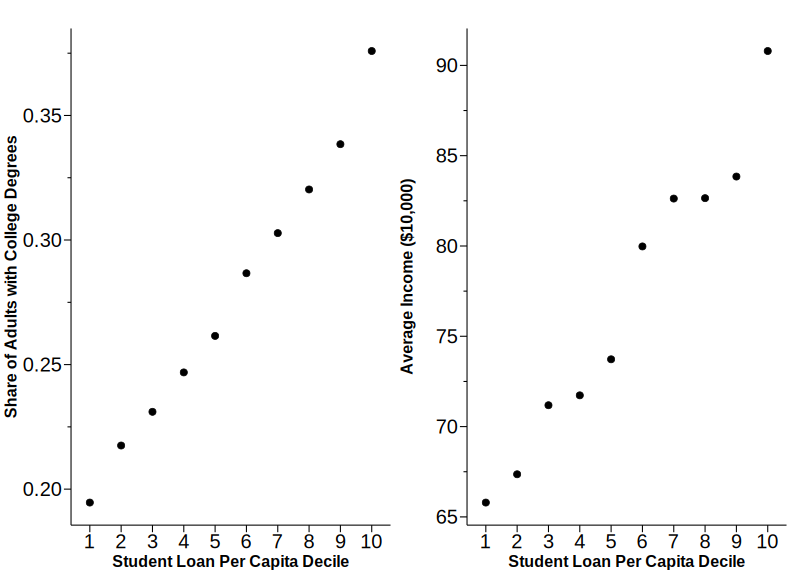
\includegraphics[width=1\textwidth,height=\textheight]{./output/figures/binscatters/binscatter-top.png}

}

\subcaption{\label{fig-binscatters-b}Aged 25--34 and Aged 65+}

\centering{

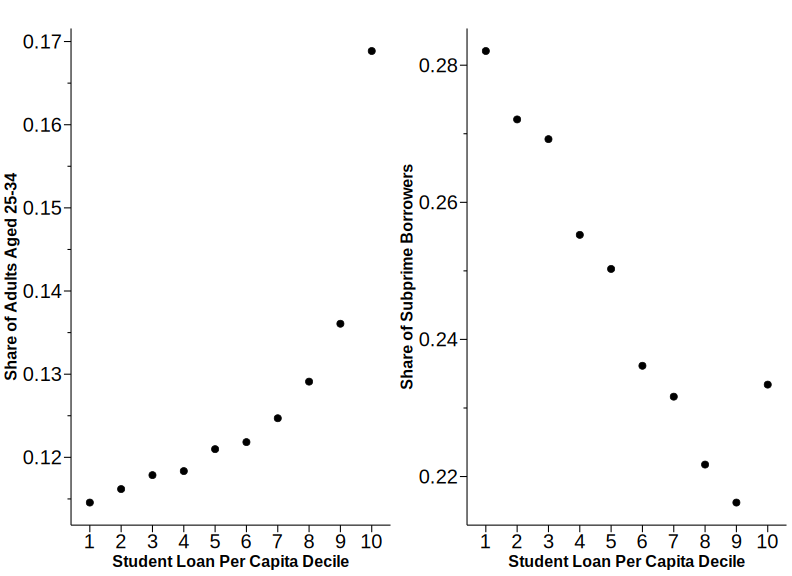
\includegraphics[width=1\textwidth,height=\textheight]{./output/figures/binscatters/binscatter-bottom.png}

}

}

\end{figure}%

\emph{Note:} This figure shows the relationship at a ZIP code level of
student loan per capita deciles against mean income, the share of
college degrees, share of individuals aged 25-34, and share of
individuals aged 65 or older. \emph{Sources}: CCP, ACS, and IRS SOI.

Because our identification relies on comparing spending in areas
differing in student loan balances, we must ensure that our
specification appropriately addresses differences in spending growth
over the period that may be driven by variation in the college share,
income distribution, and age distribution across ZIP codes. This
motivates the specification we employ, which allows spending growth to
vary flexibly based on local demographic composition and income
distribution.

\section{Empirical Methodology}\label{empirical-methodology}

We estimate a two-way fixed effects model to evaluate how the change in
ZIP code spending varied with student loan balances per adult over the
sample period January 2022 through April 2024. Specifically, we estimate
the model below, which relates the 52-week change in per capita spending
in ZIP code \(i\) in week \(t\) (\(\Delta_{52} SpendPC_{it}\)) to its
per capita student loan balances as of September 2023 (\(SLBalPC_{i}\)):
\begin{equation}\phantomsection\label{eq-event-study}{
\Delta_{52} SpendPC_{it} 
= \sum_{\tau} \beta_{\tau} \mathbf{1}_{\left\{ t = \tau \right\}}SLBalPC_{i}
+ \sum_{\tau} \gamma _\tau \mathbf{1}_{\left\{ t = \tau \right\}} \mathbf{X}_i 
+ \delta_{s(i)t} + \alpha_{i} + \varepsilon_{it}.
}\end{equation} where our main object of interest is \(\beta_\tau\),
which captures the time-varying response of consumer spending to
differential exposure to student debt per capita. Because areas with
different demographic and income characteristics may have different
spending trends over this period, and these factors are correlated with
student loan balances, we allow for trends in spending to vary with the
ZIP code's share of college-educated adults over the age of 25, as well
as the share of the population in different age and income bins. More
specifically, we control for the interaction of time dummies with the
ZIP code-level: (i) college share; (ii) share of population in various
age ranges from the 2015-2019 five year sample of the ACS; and (iii)
share of tax filing units in various adjusted gross income ranges from
the SOI, all captured in the vector \(X_i\). We weight the regression by
the ACS adult population for each ZIP code. We also include state-time
fixed effects, \(\delta_{s(i)t}\), to account for state-level
differences in spending patterns owing to weather or regional economic
trends.

Identification rests upon the assumption that, absent the student loan
payment resumption, the difference between spending growth in high- and
low-student loan ZIP codes would be zero after controlling for
potentially different spending trends by income bins, age bins, college
share, as well as state-time and ZIP code fixed effects. While we cannot
test this assumption directly, we find no evidence of differential
pre-trends between areas with more or less student debt, all else equal,
in the months prior to the resumption of student loan payments. That is,
spending growth was not significantly different for high- and
low-student loan ZIP codes prior to announcement of the payment
resumption after controlling for local income and demographic factors,
suggesting spending growth would have evolved similarly in these ZIP
codes absent the end of forbearance. \footnote{To further assess the
  validity of our empirical design, we perform a placebo test using auto
  loan debt, which was unaffected by the restart of student loan
  payments in October 2023, and which we therefore expect to be
  uncorrelated with any trends in consumer spending. To perform this
  placebo test, we re-estimate Equation~\ref{eq-event-study} using auto
  loan debt rather than student loan debt as the main independent
  variable. Reassuringly, we find no significant effect of auto loan
  debt on consumer spending during the entirety of our sample period.}

\section{Results}\label{results}

\subsection{Average effects and aggregate
implications}\label{average-effects-and-aggregate-implications}

Figure~\ref{fig-credit-png} shows the causal effect of an extra
\(\$10,000\) of student loan debt on consumer spending, measured at the
weekly level. The figure shows no significant change in consumer
spending between January 2022 and October 2023, consistent with our
assumption of conditional parallel trends before the treatment.
Following the announcement that student loan payments would resume in
June 2023, we see a gradual and persistent decline in consumer
spending.\footnote{We note that student loan payments began at different
  times for different borrowers during the month of October, hence the
  blue shaded region in Figure~\ref{fig-credit-avg} captures the window
  during which payments resumed for student loan borrowers.} The gradual
decline in consumer spending is consistent with widely-documented
features of household behavior, including inattention, consumption
commitments, and habits.

To better understand the magnitude and timing of the consumption
response, Figure~\ref{fig-credit-avg} shows the average weekly effect of
an extra \(\$10,000\) of student loan debt on consumer spending for the
post-announcement period up to the actual resumption of repayments, and
the period following the resumption of payments. The figure shows a
statistically significant consumption response following the policy
announcement in anticipation of the payment change. This anticipatory
effect is large: households reduce their spending in this
post-announcement period by about \(\$6.20\) per \(\$10,000\) of student
loan debt, compared to \(\$12.20\) in the period after payments resume.

\begin{figure}

\caption{\label{fig-credit-png}Dynamic Response of Student Debt on
Spending}

\centering{

\includegraphics[width=1\textwidth,height=\textheight]{./output/figures/event-studies/png/event-study_dec20-apr24_win99.5_credit-ma-cluster.png}

}

\end{figure}%

\emph{Note:} This figure shows the evolution of spending following the
resumption of student loan repayment for all 18,178 ZIP codes in the
filtered sample, which is obtained from running the model specified in
Equation~\ref{eq-event-study}. The gray shaded region indicates \(95\%\)
confidence bands. The solid {orange} line signifies \textbf{June 7,
2023}---the date at which Congress vetoed President Biden's plan for
student loan relief. The dotted {blue} line signifies \textbf{September
1, 2023}, which is the date at which interest began to accrue on student
loan balances. The blue-shaded region is the month of \textbf{October
2023}, the period in which monthly payments for student loan balances
restarted following the end of student loan forbearance.\\
\emph{Sources}: Verisk, CCP, ACS, and IRS SOI.

\begin{figure}

\caption{\label{fig-credit-avg}Average Response of Student Debt on
Spending}

\centering{

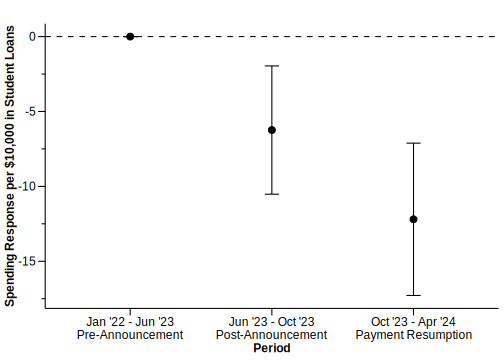
\includegraphics[width=1\textwidth,height=\textheight]{./output/figures/event-studies/png/event-study-binned-cluster.png}

}

\end{figure}%

\emph{Note:} This figure shows the evolution of spending over for 18,178
ZIP codes over three time periods: (1) ``Pre-Annoucement'', defined as
\textbf{June 7, 2023} when Congress vetoed President Biden's plan for
student loan relief; (2) ``Post-Announcement'', defined as after June 7,
2023 and up until payment resumption on \textbf{October 15, 2023}; (3)
``Payment Resumption'', defined as after October 15, 2023. We obtain the
estimates by running the model specified in
Equation~\ref{eq-event-study} using ``Pre-Announcement'' as the base
period. We include 95\% confidence bands for the ``Post-Announcement''
and ``Payment Resumption'' periods using standard errors clustered at
the ZIP code level.\\
\emph{Sources}: Verisk, CCP, ACS, and IRS SOI.

To contextualize our regression estimates, consider the following
back-of-the-envelope calculations for the implied partial equilibrium
effect of the end of student loan forbearance on the level of nominal
PCE and GDP. We begin with our estimate of the weekly effect of the
resumption of student loan payments on spending: \$12.20 per \$10,000 of
balances. This estimate translates to an annualized reduction in
spending of {[}\$630{]} per year for every \$10,000 in student loan
balances. These numbers imply an annualized cutback in spending of
\$1590 for the median student loan borrower and \$2980 for the
mean.\footnote{These numbers are based on the median debt level for a
  borrower in the 2022 Survey of Consumer Finances, about \$25,000 and
  the mean student loan debt per borrower, about \$47,000.} Given that
we find about \$1.25 trillion of eligible student debt at the time the
policy ended, our estimates imply that the resumption of student loan
payments reduced consumer spending by \$80 billion at an annual rate,
which is roughly 0.3 percent of GDP or 0.4 percent of personal
consumption expenditures in the first quarter of 2024.\footnote{Note
  that while our estimates may include very local (i.e., within-ZIP
  code) general equilibrium effects, these estimates and do not consider
  the numerous national general equilibrium effects that could either
  offset or magnify this change in aggregate demand.}

While much of the literature on spending responses to policy changes
focuses on measuring the marginal propensity to consume (MPC) from a
shock, our results do not directly translate to comparable figures. In
particular, because servicers were not required to report required
payments to credit bureaus for at least a year after the end of
forbearance, the CCP provides reliable measures of debt levels, but not
required payments in the quarters immediately after payment resumption.
However, we are able to translate the spending response to debt into an
MPC by utilizing information after servicers began reporting required
payments and delinquencies in 2024:Q3. Overall, these data imply an
aggregate payment-to-balance ratio of roughly 5.75 percent per
year\footnote{Because of changes in Income Driven Repayment plans and
  deferrals due to the SAVES Act in 2024, we opt to utilize data after
  reporting resumed rather than older data on payments. We find the
  ratio of annual required payments to balances for federal loans in the
  CCP where required payments are positive was 10.4 percent per year in
  2024:Q3 through 2025:Q1. In addition, roughly 30 percent of federal
  loans by balance had required payments of 0. (Zero required payments
  reflect a combination of grace periods/deferrals, in-school status,
  and forbearance. See: https://www.congress.gov/crs-product/IF12896)}.
Applying these ratios to our estimated effects per-dollar-of-debt, we
find an MPC just over 1 dollar of consumption per dollar of
payment---somewhat high but not out of the realm of other estimates of
MPCs out of permanent income shocks.\footnote{See, for example, Gelman
  et al. (2023).}

Our study provides the first evidence on the response in consumer
spending following the restart of student loan repayment using actual
spending data, and we find evidence that the end of forbearance caused
meaningful drag on aggregate demand. Our results imply somewhat larger
responses than other studies that did not have actual spending data.
Chakrabarti, Mangrum, et al. (2023), for example, conduct a survey where
they ask borrowers how they plan to adjust their spending between
October and December 2023 due to the resumption of student loan
repayment. Those authors find that borrowers expect to reduce
consumption by around \$56 per month. Our numbers suggest that the
effect of the resumption of payments may have been larger than their
survey suggested; we find that the median borrower reduced consumption
by about \$130 per month.

\section{Conclusion}\label{conclusion}

In this note, we estimate how household spending changed following the
end of student loan forbearance. To do this, we exploit ZIP code-level
variation in student loan balances, merged with high-frequency data on
ZIP code household spending. Our estimates imply that households reduced
spending meaningfully following the resumption of required payments in
October 2023. The average consumer cut back spending by \$1590 per year.
Further, a partial-equilibrium exercise suggests that the policy was
supporting consumer spending by \$80 billion at an annual rate.

\section*{References}\label{references}
\addcontentsline{toc}{section}{References}

\phantomsection\label{refs}
\begin{CSLReferences}{1}{0}
\bibitem[\citeproctext]{ref-amromin2016education}
Amromin, Gene, and Janice Eberly. 2016. {``Education Financing and
Student Lending.''} \emph{Annual Review of Financial Economics} 8 (1):
289--315.

\bibitem[\citeproctext]{ref-armona2022student}
Armona, Luis, Rajashri Chakrabarti, and Michael F Lovenheim. 2022.
{``Student Debt and Default: The Role of for-Profit Colleges.''}
\emph{Journal of Financial Economics} 144 (1): 67--92.

\bibitem[\citeproctext]{ref-chakrabarti2023tuition}
Chakrabarti, Rajashri, Vyacheslav Fos, Andres Liberman, and Constantine
Yannelis. 2023. {``Tuition, Debt, and Human Capital.''} \emph{The Review
of Financial Studies} 36 (4): 1667--1702.

\bibitem[\citeproctext]{ref-chakrabarti2023borrower}
Chakrabarti, Rajashri, Daniel Mangrum, Sasha Thomas, and Wilbert Van der
Klaauw. 2023. {``Borrower Expectations for the Return of Student Loan
Repayment.''} Federal Reserve Bank of New York.

\bibitem[\citeproctext]{ref-dinerstein2024debt}
Dinerstein, Michael, Constantine Yannelis, and Ching-Tse Chen. 2024.
{``Debt Moratoria: Evidence from Student Loan Forbearance.''}
\emph{American Economic Review: Insights} 6 (2): 196--213.
\url{https://doi.org/10.1257/aeri.20230032}.

\bibitem[\citeproctext]{ref-field2009educational}
Field, Erica. 2009. {``Educational Debt Burden and Career Choice:
Evidence from a Financial Aid Experiment at NYU Law School.''}
\emph{American Economic Journal: Applied Economics} 1 (1): 1--21.

\bibitem[\citeproctext]{ref-gelman2023AEJ}
Gelman, Michael, Yuriy Gorodnichenko, Shachar Kariv, Dmitri Koustas,
Matthew D. Shapiro, Dan Silverman, and Steven Tadelis. 2023. {``The
Response of Consumer Spending to Changes in Gasoline Prices.''}
\emph{American Economic Journal: Macroeconomics} 15 (2): 129--60.
\url{https://doi.org/10.1257/mac.20210024}.

\bibitem[\citeproctext]{ref-GossMangrumScaley2024}
Goss, Jacob, Daniel Mangrum, and Joelle Scally. 2024. {``Assessing the
Relative Progressivity of the Biden Administration's Federal Student
Loan Forgiveness Proposal.''} \emph{Education Finance and Policy} 19
(4): 716--33. \url{https://doi.org/10.1162/edfp_a_00429}.

\bibitem[\citeproctext]{ref-jacob2024value}
Jacob, Brian A, Damon Jones, and Benjamin J Keys. 2024. {``The Value of
Student Debt Relief and the Role of Administrative Barriers: Evidence
from the Teacher Loan Forgiveness Program.''} \emph{Journal of Labor
Economics} 42 (S1): S261--92.

\bibitem[\citeproctext]{ref-krishnan2019cost}
Krishnan, Karthik, and Pinshuo Wang. 2019. {``The Cost of Financing
Education: Can Student Debt Hinder Entrepreneurship?''} \emph{Management
Science} 65 (10): 4522--54.

\bibitem[\citeproctext]{ref-lochner2016student}
Lochner, Lance, and Alexander Monge-Naranjo. 2016. {``Student Loans and
Repayment: Theory, Evidence, and Policy.''} In \emph{Handbook of the
Economics of Education}, 5:397--478. Elsevier.

\bibitem[\citeproctext]{ref-luo2019assets}
Luo, Mi, and Simon Mongey. 2019. {``Assets and Job Choice: Student Debt,
Wages and Amenities.''}

\bibitem[\citeproctext]{ref-ACS_NHGIS}
Manson, Steven, Jonathan Schroeder, David Van Riper, Katherine Nowles,
Tracy Kugler, Finn Roberts, and Steven Ruggles. 2024. {``IPUMS National
Historical Geographic Information System: Version 19.0 {[}Dataset{]}.''}
\url{https://doi.org/10.18128/D050.V19.0}.

\bibitem[\citeproctext]{ref-mezza2020student}
Mezza, Alvaro, Daniel Ringo, Shane Sherlund, and Kamila Sommer. 2020.
{``Student Loans and Homeownership.''} \emph{Journal of Labor Economics}
38 (1): 215--60.

\bibitem[\citeproctext]{ref-mian2023partisan}
Mian, Atif, Amir Sufi, and Nasim Khoshkhou. 2023. {``Partisan Bias,
Economic Expectations, and Household Spending.''} \emph{The Review of
Economics and Statistics} 105 (3): 493--510.
\url{https://doi.org/10.1162/rest_a_01056}.

\bibitem[\citeproctext]{ref-mueller2019rise}
Mueller, Holger M, and Constantine Yannelis. 2019. {``The Rise in
Student Loan Defaults.''} \emph{Journal of Financial Economics} 131 (1):
1--19.

\bibitem[\citeproctext]{ref-rothstein2011constrained}
Rothstein, Jesse, and Cecilia Elena Rouse. 2011. {``Constrained After
College: Student Loans and Early-Career Occupational Choices.''}
\emph{Journal of Public Economics} 95 (1-2): 149--63.

\bibitem[\citeproctext]{ref-Verisk}
Verisk. 2024. {``Verisk Commerce Signals Spend Tracker.''}

\bibitem[\citeproctext]{ref-yannelis2022student}
Yannelis, Constantine, and Greg Tracey. 2022. {``Student Loans and
Borrower Outcomes.''} \emph{Annual Review of Financial Economics} 14
(1): 167--86.

\end{CSLReferences}




\end{document}
